\chapter{基于神经网络预测太阳黑子}\label{chap:ml_sunspot}

\section{引言}\label{sec:ss_intro}

太阳活动是太阳大气中局部区域各种不同活动现象的总称,包括太阳黑子、日珥、光斑、谱斑、耀斑、太阳风和日冕质量抛射等。处于活动剧烈期的太阳会辐射出大量紫外线、x射线、粒子流和强射电波,导致地球上出现极光、磁暴和电离层扰动等现象。太阳活动对地球的影响有以下几个方面\citep{jie2012prediction}:
\begin{itemize}
  \item \textbf{地球大气层}。地球大气层在太阳的辐射下形成电离层,无线电波依靠电离层的反射向远距离传播。当太阳活动剧烈时,在向阳的半球电离层容易衰减甚至中断。
  \item \textbf{地球气候}。统计上,太阳活动周期与地球气候的关系也比较明显,其作用机制目前还不清楚。太阳活动达到高峰时,地球上太平洋热带及亚热带地区气温升高、海水加速蒸发、西太平洋热带海域的降雨增多,东太平洋热带海域气温降低。
  \item \textbf{地球磁场}。太阳活动剧烈时地球磁场会产生磁暴现象。
  \item \textbf{航天活动}。大耀斑出现时射出的高能量质子,对航天飞行、卫星设备、太阳能电池等有极大的破坏性。
\end{itemize}

太阳黑子是太阳活动的基本标志,是太阳活动现象过程中很容易观测到的特征之一。由太阳大气中的电磁过程引起。时烈时弱,平均以11或22年为周期。太阳黑子能够反应太阳活动的剧烈程度,通常数量越多,太阳活动越频繁。太阳黑子出现在太阳光球上的黑暗区域,肉眼可见。太阳黑子可以成群出现,也可以是单个孤立的本影,周围有半影。本影是一个黑暗的中心区域,而半影是一个不太黑暗的区域。太阳黑子的产生是由于在太阳内部产生的强磁场,\citet{noyes2013sun}详细阐述了太阳黑子的产生机制。

目前,有关太阳黑子的记录可长达400多年,其时间序列数据显示出周期性震荡。通过从预测结果中获得信息,有助于人类做出提前的准备,可以降低太阳黑子对地球和人类的影响。

传统意义上,基于物理机制的预测模型(例如,前兆,动态模型,混沌理论\citep{jie2012prediction})和统计预测模型(比如,自回归移动平均模型)已经被广泛应用于太阳黑子时间序列预测。然而,这些模型都有一个前提假设,时间序列是从线性过程产生的,难以有效地抓住非高斯性、非稳态性和非线性的时间序列关系\citep{jiang2011sunspot,arlt2015solar}。
近些年来,机器学习在太阳黑子预测中的应用非常流行\citep{pala2019forecasting},可拟合非常复杂的函数,具有强大的容错能力。\citet{zhao2008prediction}使用径向基神经网络预测未来4个月的平滑月均太阳黑子数,发现相对误差控制在38\%以内,而且误差会随着预测时间的延长而逐渐增加。\citet{ding2012prediction}基于反向传播神经网络(Backpropagation Neural Network,简称BPNN)预测平滑月均太阳黑子面积,发现相对误差不超过5\%。\citet{li2018hybrid}在预测太阳黑子数时,使用了BPNN及其变种的神经网络,发现组合的神经网络强于BPNN,RMSE为1.7117,MAPE为0.0435。

尽管很多学者利用年/月均太阳黑子时间序列数据预测未来一个太阳周(尤其是第25太阳周)的峰值,却没有得出一个统一的结论。对黑子数而言,第23太阳周太阳黑子数峰值出现在2001年9月,其值为238.2;第24太阳周太阳黑子数峰值出现在2014年2月,其值为146.1。对于太阳黑子面积,第23太阳周太阳黑子峰值为2171.7,出现在2001年9月;第24太阳周太阳黑子峰值为1439.82,出现在2014年2月。对于第25太阳周太阳黑子强度,可分为以下几种结论:
\begin{enumerate}
  \item 与第24太阳周相比,第25太阳周太阳黑子更强。也就是说,太阳黑子可能不会大幅减弱,甚至可能扭转太阳活动大幅减弱的趋势。\citet{mcintosh2020overlapping}基于磁活动周期的物理模型,预测到第25太阳周是有史以来观察到的最强的太阳黑子周期之一,峰值为233。\citet{pesnell2018effects}采用na{\"\i}ve方法,得到第25太阳周的太阳黑子数为180\pm 60。
  \item 与第24太阳周相比,第25太阳周太阳黑子基本与之持平。\citet{bisoi2020another}得出第25太阳周太阳黑子数峰值为$\sim$131-134,出现在2025年7月。\citet{singh2019prediction}得出第25太阳周太阳黑子数峰值为124$\sim$11,出现在2024年2月。\citet{hiremath2008prediction}预测未来$\sim$170年的太阳黑子变化,发现第24和25太阳周的太阳黑子数均为$\sim$110。\citet{bhowmik2018prediction}使用太阳表面通量传输模型和太阳内部动力模型,基于年均太阳黑子数据集,得到第25太阳周的太阳黑子数为$\sim$118,发生在$\sim$2024年。
  \item 与第24太阳周相比,第25太阳周太阳黑子更弱。\citep{kitiashvili2020application}使用同步磁图发现第25太阳周的最大太阳黑子数为$\sim$50(发生在2024年或2025年),该数值将甚至少于Dalton最低点期间的太阳黑子数,可能与Maunder最低点相当。
\end{enumerate}

总之,无论最终模型的表现效果如何,目前很难对未来第25太阳周太阳黑子活动的非线性动态特征(太阳黑子峰值和太阳周持续时间)的进行精准预测。太阳黑子时间序列具有非平稳性、非高斯性、非线性特征,预测太阳黑子变化颇具挑战性。通过机器学习探索太阳黑子变化趋势,有助于理解太阳活动的机制。鉴于预测未来第25太阳周太阳黑子活动难以取得一致性,我们尝试预测未来1个月至几个太阳周的太阳黑子变化,探索在哪种情况下能够较为精准地预测出太阳黑子数。

本章节结构安排如下。第\ref{sec:ss_data_method}节描述了太阳黑子数量和面积的时间序列以及两者在变化趋势上的差异、数据的预处理过程以及使用的模型。第\ref{sec:ss_result}节描述太阳黑子变化的试验过程,并将试验结果进行可视化。第\ref{sec:ss_conclusion}节对预测太阳黑子动态变化进行了总结,并对下一步研究进行了展望。

\section{数据与方法}\label{sec:ss_data_method}

本节首先介绍了太阳黑子数量和面积的时间序列以及两者长期的变化趋势。接着,介绍原始数据集进行预处理的过程,包括生成监督学习数据集、数据集划分、归一化处理等。然后,选取几种不同结构的神经网络训练处理后的数据。

\subsection{数据描述}\label{sec:ss_dataset}

本章采用两种时间序列数据集。第一类为月均太阳黑子数(Monthly Mean Total Sunspot Number,简称MSSN),来自SILSO(Sunspot Index and Long-Term Solar Observation)网站\footnote{数据来源:WDC-SILSO, Royal Observatory of Belgium, Brussels, \href{http://sidc.be/silso/datafiles}{http://sidc.be/silso/datafiles}}发布的太阳黑子2.0版本。MSSN数据集跨越了273年(从1749年1月至2021年8月), 包含3272条记录。截至目前,MSSN数据集已经涵盖了24个太阳周。表\ref{tab:ss_max_min}展示了这24个太阳周太阳黑子数量、峰值和谷值出现时间。第1太阳周为1755年2月至1766年5月,目前正处于第25太阳周的起始阶段\footnote{参考:\href{www://sidc.be/silso/cyclesmm}{www://sidc.be/silso/cyclesmm}}。图\ref{fig:ss_number_series}使用了1749年1月至2021年8月期间月均太阳黑子数时间序列数据,绘制出太阳黑子数的变化趋势图。图\ref{fig:ss_number_series}显示,MSSN数据集的分布均右偏的。\citet{panigrahi2021forecasting}指出,MSSN数据集的峰度大于3。鉴于MSSN数据集呈现复杂的非高斯型分布,因此较难预测出太阳黑子的变化趋势。

\begin{table}[!htbp]
  \centering
  \bicaption{太阳黑子数量、峰值和谷值出现时间。}{Solar minimum and maximum timings and amplitudes of sunspot numbers.}
  \label{tab:ss_max_min}
  \footnotesize
  \renewcommand{\arraystretch}{1}
  \begin{tabular}{cccccccc}
    \toprule
    \multicolumn{1}{c}{}&\multicolumn{2}{c}{谷值}&
    \multicolumn{2}{c}{峰值}& \multicolumn{3}{c}{时间(年)}\\
    \cmidrule(lr){2-3} \cmidrule(lr){4-5} \cmidrule(lr){6-8} \noalign{\smallskip}
    \multicolumn{1}{c}{太阳周} & 日期 & 黑子数 & 日期 & 黑子数 & 上升 & 下降 & 最小值到最小值\\ 
    \midrule 
    1 & 1755.204 & 14.0 & 1761.455 & 144.1 & 6.251 & 5.000 & 11.251 \\
    2 & 1766.455 & 18.6 & 1769.707 & 193.0 & 3.252 & 5.748 & 9.000 \\
    3 & 1775.455 & 12.0 & 1778.371 & 264.3 & 2.916 & 6.337 & 9.253 \\
    4 & 1784.708 & 15.9 & 1788.124 & 235.3 & 3.416 & 10.164 & 13.580 \\
    5 & 1798.288 & 5.3 & 1805.123 & 82.0 & 6.835 & 5.835 & 12.670 \\
    6 & 1810.958 & 0.0 & 1816.373 & 81.2 & 5.415 & 6.998 & 12.413 \\
    7 & 1823.371 & 0.2 & 1829.874 & 119.2 & 6.503 & 4.000 & 10.503 \\
    8 & 1833.874 & 12.2 & 1837.204 & 244.9 & 3.330 & 6.334 & 9.664 \\
    9 & 1843.538 & 17.6 & 1848.124 & 219.9 & 4.586 & 7.834 & 12.420 \\
    10 & 1855.958 & 6.0 & 1860.124 & 186.2 & 4.166 & 7.080 & 11.246 \\
    11 & 1867.204 & 9.9 & 1870.623 & 234.0 & 3.419 & 8.335 & 11.754 \\
    12 & 1878.958 & 3.7 & 1883.958 & 124.4 & 5.000 & 6.246 & 11.246 \\
    13 & 1890.204 & 8.3 & 1894.042 & 146.5 & 3.838 & 8.000 & 11.838 \\
    14 & 1902.042 & 4.5 & 1906.123 & 107.1 & 4.081 & 7.500 & 11.581 \\
    15 & 1913.623 & 2.5 & 1917.623 & 175.7 & 4.000 & 6.000 & 10.000 \\
    16 & 1923.623 & 9.4 & 1928.290 & 130.2 & 4.667 & 5.417 & 10.084 \\
    17 & 1933.707 & 5.8 & 1937.288 & 198.6 & 3.581 & 6.836 & 10.417 \\
    18 & 1944.124 & 12.9 & 1947.371 & 218.7 & 3.247 & 6.917 & 10.164 \\
    19 & 1954.288 & 5.1 & 1958.204 & 285.0 & 3.916 & 6.587 & 10.503 \\
    20 & 1964.791 & 14.3 & 1968.874 & 156.6 & 4.083 & 7.332 & 11.415 \\
    21 & 1976.206 & 17.8 & 1979.958 & 232.9 & 3.752 & 6.749 & 10.501 \\
    22 & 1986.707 & 13.5 & 1989.874 & 212.5 & 3.167 & 6.750 & 9.917 \\
    23 & 1996.624 & 11.2 & 2001.874 & 180.3 & 5.250 & 7.084 & 12.334  \\
    24 & 2008.958 & 2.2 & 2014.288 & 116.4 & 5.330 & — & —  \\
    平均值 & 9.29 &  & 178.7 & 4.33 & 6.74 & 11.03  \\
    标准差 & 5.70 &  & 57.76 & 1.11 & 1.24 & 1.18 \\
    中值 & 9.65 &  & 183.3 & 4.08 & 6.75 & 11.25 \\
    \bottomrule
  \end{tabular}
\end{table}

\begin{figure}[!htbp]
    \centering
    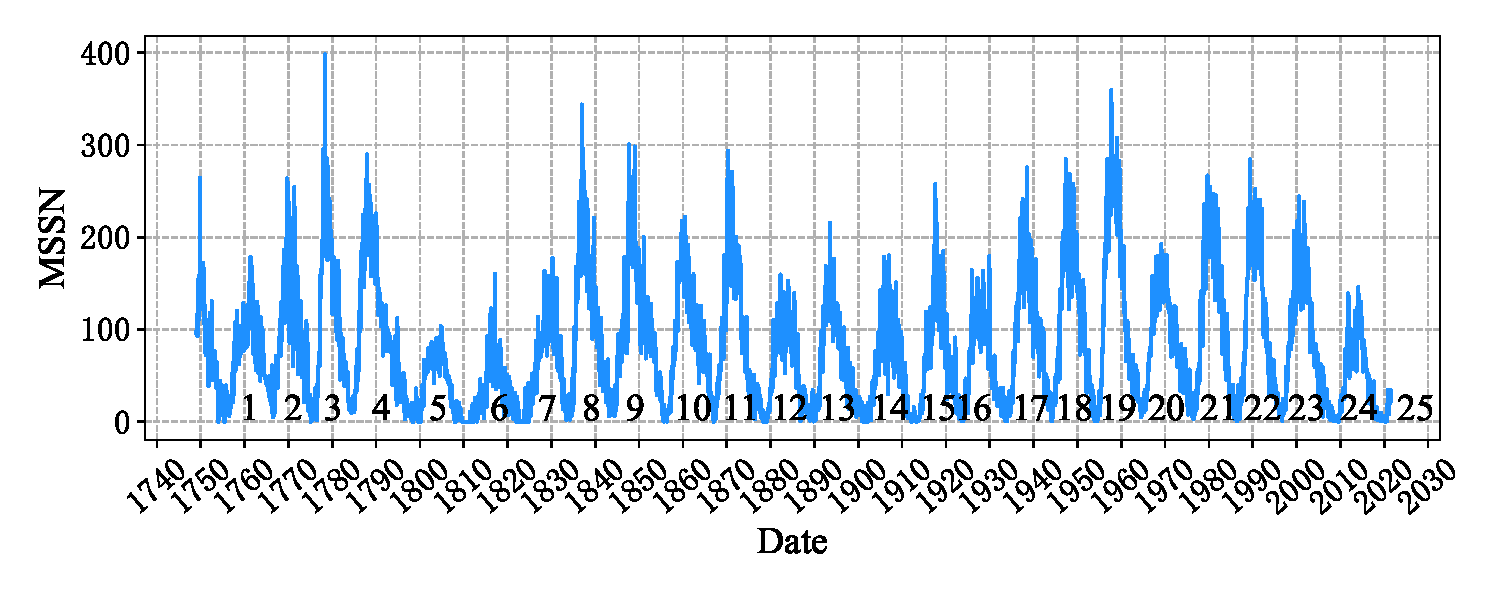
\includegraphics[width=\textwidth]{Img/chap5_ss/ss_number_series.pdf}
    \vspace{-1.4cm}
    \bicaption{1949年至2021年月均太阳黑子数时间序列数据集。}{Monthly mean total sunspot number time series between 1749 and 2021.}
    \label{fig:ss_number_series}
  \end{figure}

第二类数据集为太阳黑子面积(Sunspot Area,简称SSA)。SSA数据集来自Lisa Upton和DavidHathaway提供的网站\footnote{参考:\href{http://solarcyclescience.com/activeregions.html}{http://solarcyclescience.com/activeregions.html}},该数据集可用来预测太阳黑子面积和太阳黑子蝴蝶图。\citet{hathaway2015solar}指出,SSA数据集也是一个好的长时间序列的太阳磁活动指标,跟MSSN数据集一样,同样也可以应用在预测太阳周期。SSA数据集跨越了147年(从1874年5月1日至2021年8月7日),包含247693条记录,因此数据集包含了13个完整的太阳周。同MSSN数据集相比,SSA数据集还涵盖了黑子发生的位置信息。因此SSA数据集在理解长期太阳磁活动和变化非常重要。如图\ref{fig:ss_butterfly}所示,根据1874年至2021年间太阳黑子面积随着时间和纬度的变化,我们绘制出了蝴蝶图。在每个太阳周早期,太阳黑子出现在高纬度地区,然后向赤道方向移动。

\begin{figure}[!htbp]
  \vspace{-0.3cm}
  \centering
  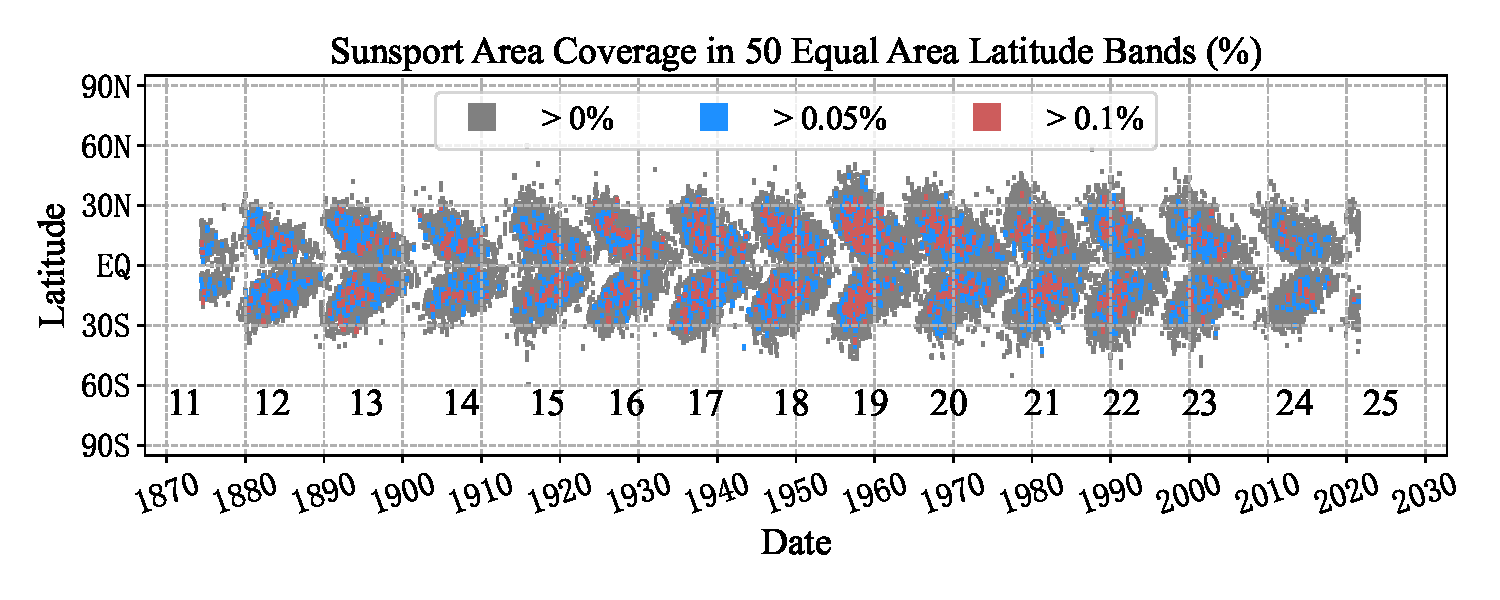
\includegraphics[width=\textwidth]{Img/chap5_ss/ss_butterfly.pdf}
  \vspace{-1.4cm}
  \bicaption{1949年至2021年期间太阳黑子面积随时间和纬度变化的蝴蝶图。}{Butterfly diagram of sunspot area, which marks the latitude of sunspot locations as a function of time between 1749 and 2021.}
  \label{fig:ss_butterfly}
\end{figure}

为保持太阳黑子数和面积在时间上的一致性,将SSA数据集中的太阳黑子面积按月均,得到MSSA(Monthly SSA)数据集。将MSSN和MSSA两种时间序列数据集绘制在同一张图中,可显示太阳黑子数和太阳黑子面积之间的关系。如图\ref{fig:ss_number_area}所示,我们截取了MSSA在1874年至2021年的种数据集,纵轴按照不同尺度标准绘制太阳黑子数和太阳黑子面积的变化趋势。在重叠的时间范围内,太阳黑子数和面积在太阳活动强度和发生时间上存在高度的关联性。

\begin{figure}[!htbp]
  \vspace{-0.3cm}
  \centering
  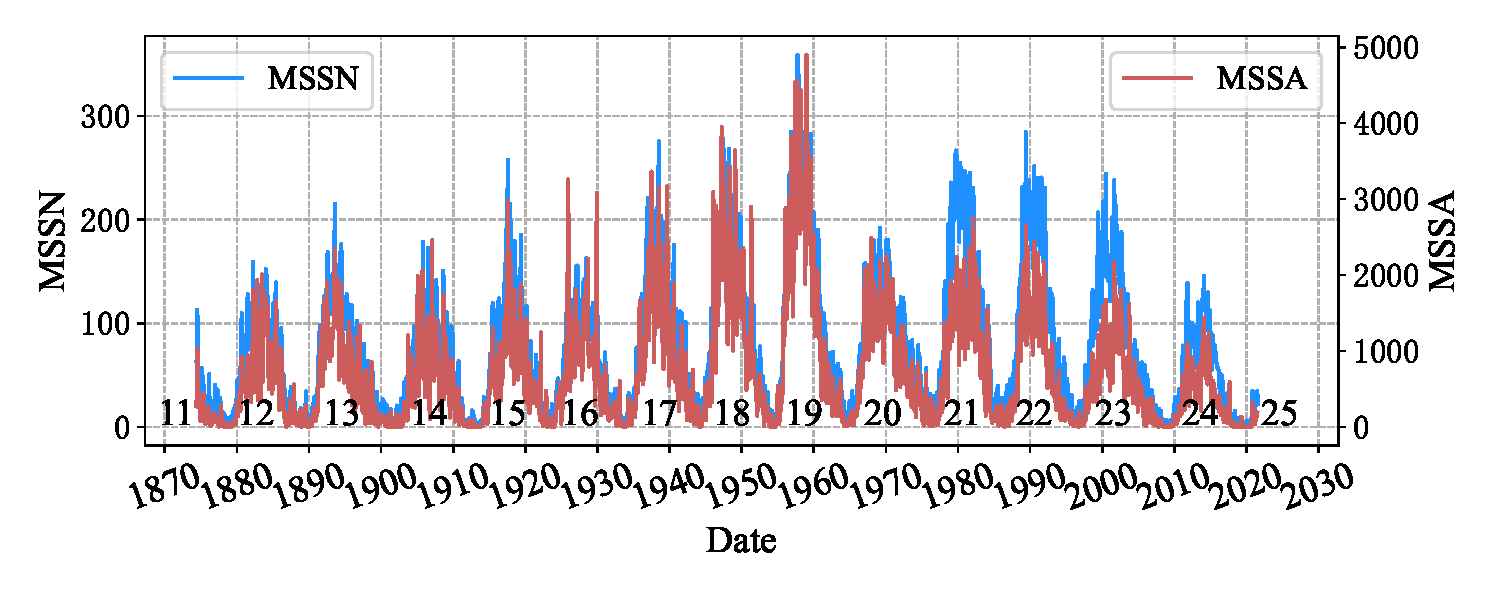
\includegraphics[width=\textwidth]{Img/chap5_ss/ss_number_area.pdf}
  \vspace{-1.4cm}
  \bicaption{1874年至2021年间月均的太阳黑子数和月均太阳的黑子面积。}{Monthly mean sunspot numbers and monthly mean sunspot areas from 1874 to 2021.}
  \label{fig:ss_number_area}
\end{figure}

\subsection{方法描述}\label{subsec:ss_method}

本小节围绕预处理方法和机器学习方法展开。这里使用不同种类的神经网络模拟太阳黑子的动态变化特征。为了更精准地捕获太阳黑子变化趋势,我们使用了近几百年来观测到的太阳黑子数量/面积,试图从历史观测数据中提取关键信息,预测未来太阳活动。首先,将原始观测数据集转化为监督学习时间序列数据集。太阳黑子强度可以从长期历史记录中预测,依赖历史的时间长度从1个月到几个太阳周不等。太阳黑子变化趋势可以被近似表达为:
\begin{equation}
  \label{eq:ss_sunspot_equation}
  S(t,t+\Delta,\ldots,t+n\Delta)=S[P(t-\Delta),S(t-2\Delta),\ldots,S(t-m\Delta t)].
\end{equation}
其中,$\Delta t$代表样本的采样间隔,本研究中将采样间隔设为1个月。$S(t,t+\Delta,\ldots,t+n\Delta)$代表预测未来$n$个月的太阳黑子强度,$S(t-\Delta t),S(t-2\Delta t),\ldots,S(t-m\Delta)$代表历史$m$个月的太阳黑子强度。

通过第\ref{sec:ml_slide}节的滑动窗口法,我们可以将原始太阳黑子数量数据集$\text{MSSN}_{\text{raw}}$转换为监督学习数据集$\text{MSSN}_{\text{supervised}}$。紧接着,我们将数据集$\text{MSSN}_{\text{supervised}}$分割为训练集$\text{MSSN}_{\text{train}}$和测试集$D_{\text{test}}$,分割比例为0.8:0.2,详见第\ref{sec:ml_split}节。在训练集$\text{MSSN}_{\text{train}}$和测试集$\text{MSSN}_{\text{test}}$被使用之前,我们需要对两者分别进行归一化处理(第\ref{sec:ml_scaler}节),得到了训练集$\text{MSSN}^T_{\text{train}}$和测试集$\text{MSSN}^T_{\text{test}}$。MSSA数据集也会进行类似的操作。

因为太阳活动的复杂性,太阳黑子时间序列呈现出复杂的非线性、非高斯型分布风特征。式\ref{eq:ss_sunspot_equation}明确指出,模型的输入是历史记录的太阳黑子数量/面积,输出为接未来的太阳黑子数量/面积。第\ref{sec:ml_cnn}节和第\ref{sec:ml_lstm}节提到,LSTM-RNN和1DCNN均适用于时间序列数据。因此,这里我们选择了LSTM-RNN和1DCNN。考虑到LSTM-RNN和1DCNN对处理时间序列数据有着不同的优势,我们综合这两种网络中的特点,得到LSTM-1DCNN。

\section{试验结果与分析}\label{sec:ss_result}

相较于32年的泉流量时间序列数据集,太阳黑子数据集记录的时间相对较长。MSSN数据集跨越了273年,MSSA数据集跨越了147年。因为本研究的目标是利用实验观测数据评估模型的预测能力。引言\ref{sec:ss_intro}提到,太阳黑子变化存在周期性,平均为$\sim$11年或$\sim$22年。这里我们考虑输入时间窗口为1、72、132、264,评估不同输入时间窗口对模型的影响。每个输入响应可以表示如下:
\begin{equation}
  \label{eq:ss_input}
  \begin{split}
    I_{-k}=[S(t),S(t-1),\ldots,S(t-k+1)].
  \end{split}
\end{equation}
其中,$k=1,72,132,264$。

通常我们会关注未来一个太阳周内的太阳黑子强度。在泉流量动态试验过程中,我们发现及其学习预测较长的时间序列会产生一定的误差,为了预测第25太阳周的峰值,因此可以将输出窗口设置为72。将未来72个月太阳黑子最大的值定义为第25太阳周的峰值。每个输出响应可以表示如下:
\begin{equation}
  \label{eq:ss_output}
  O_{+f}=[O(t+1),O(t+2),\ldots,O(t+f)].
\end{equation}
其中,$f=1,72$。

这里,我们简要介绍不同的超参数配置。所有模型的输入节点数$k$由输入窗口决定,输出节点数$f$由输出窗口决定。以下是所有神经网络通用的超参数。训练经过1000回合,网络每层均会使用ReLU激活函数。批量训练数据量设为132。Adam方法作为优化器。学习率初始值设为$10^{-3}$。同时训练次数每增加10次,学习率会减小$1-10^{-6}$倍,这样逐步减小学习率能够防止模型陷入局部极小值。为防止过拟合现象,所有试验均使用“早停”方案,即100次迭代后,若测试集的MSE值没有下降,则停止训练。

\subsection{预测未来1个月太阳黑子强度}\label{sec:ss_result_1}

我们采用了两层架构的LSTM-RNN和1DCNN,LSTM-1DCNN采用了三层。因各种网络具有的独特性质,在设置以下超参数时会有所差异。针对LSTM-RNN,隐藏层含LSTM神经元,最后一层为全连接层。隐藏层的节点数设为32,输出层为全连接层。针对1DCNN,隐藏层为1维卷积层,过滤器个数、过滤器大小、步长分别为32、3、2。卷积层后连接了最大池化层,池化大小为2,步长为1。最后一层为全连接层。针对LSTM-1DCNN,第一、二层均含有LSTM神经元,神经元个数分别为64和32。第三层为1维卷积层,过滤器个数、过滤器大小、步长分别为16、3、1。最后一层为全连接层。 

讨论输出时间窗口为1个月的太阳黑子强度。表\ref{tab:ss_number_out_1}展示了使用不同模型(LSTM-RNN、1DCNN和LSTM-1DCNN)、不同输入窗口(1、72、132、264)未来1个月太阳黑子数量效果指标。表\ref{tab:ss_out_1}第一行展示了预测的未来太阳黑子数量。就网络性能而言,LSTM-1DCNN性能略优于LSTM-RNN和1DCNN。就输入窗口而言,历史72个月的太阳黑子数量作为时间窗口所得到的模型是最优的。当输入时间窗口为72个月$O_{-72}$时,LSTM-RNN的拟合指标为MSE$=\SI{0.0031}{}$, RMSE$=\SI{0.0554}{}$,预测2021年9月的太阳黑子数为$\SI{37.9250}{}$;1DCNN的拟合指标为MSE$=\SI{0.0041}{}$, RMSE$=\SI{0.0640}{}$,预测2021年9月的太阳黑子数为$\SI{31.6609}{}$;LSTM-1DCNN的拟合指标为MSE$=\SI{0.0030}{}$, RMSE$=\SI{0.547}{}$,预测2021年9月的太阳黑子数为$\SI{41.1549}{}$。

\begin{table}[!htbp]
  \centering
  \bicaption{不同模型、不同输入窗口预测未来1个月太阳黑子数量的测试集效果指标。}{The indicators of testing set for predicting the next monthly sunspot numbers by different models with different input windows.}
  \label{tab:ss_number_out_1}
  \footnotesize
  \renewcommand{\arraystretch}{1}
  \begin{tabular}{ccccc}
    \toprule
    \multirow{2}{*}{模型} & \multirow{2}{*}{$I_{-k}$-[节点或过滤器数]-$O_{+f}$} & \multicolumn{2}{c}{验证集}\\
    \cmidrule(lr){3-4}
    \noalign{\smallskip}
    & & MSE & RMSE\\
    \midrule 
    LSTM-RNN & 1-[32]-1 & 0.0037 & 0.0609 \\
    LSTM-RNN & 72-[32]-1 & \textbf{0.0031} & \textbf{0.0554} \\
    LSTM-RNN & 132-[32]-1 & 0.0032 & 0.0568 \\
    LSTM-RNN & 264-[32]-1 & 0.0034 & 0.0584 \\
    \hline
    1DCNN & 72-[32]-1 & \textbf{0.0041} & \textbf{0.0640} \\
    1DCNN & 132-[32]-1 & 0.0042 & 0.0647 \\
    1DCNN & 264-[32]-1 & 0.0043 & 0.0658 \\
    \hline
    LSTM-1DCNN & 72-[64-32-16]-1 & \textbf{0.0030} & \textbf{0.547} \\
    LSTM-1DCNN & 132-[64-32-16]-1 & 0.0034 & 0.0581 \\
    LSTM-1DCNN & 264-[64-32-16]-1 & 0.0035 & 0.0594 \\
    \bottomrule
  \end{tabular}
\end{table}

\begin{figure}[!htbp]
  \centering
  \begin{subfigure}[b]{1.0\textwidth}
    \caption{LSTM-RNN} 
    \vspace{-0.35cm}
    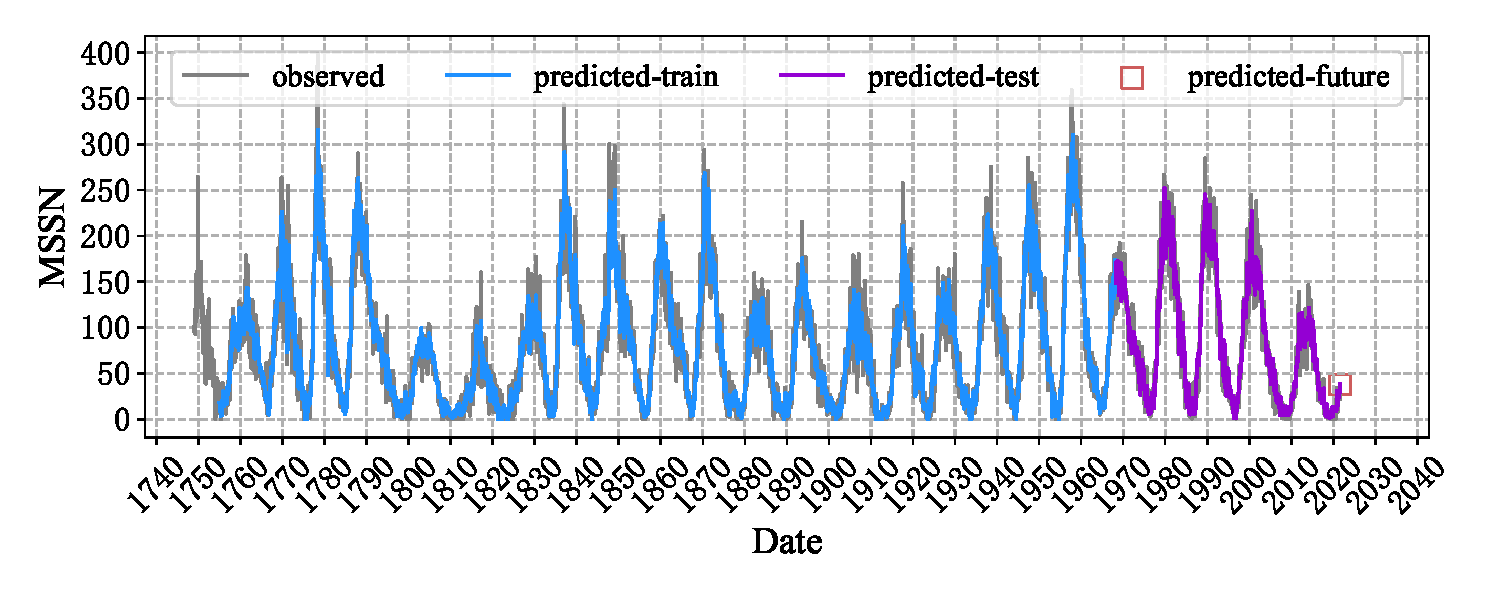
\includegraphics[width=\textwidth]{Img/chap5_ss/ssn_series_in_72_out_1_lstm.pdf}
    \label{fig:ssn_series_in_72_out_1_lstm}
  \end{subfigure}    \\
  \vspace{-1cm}
  \begin{subfigure}[b]{1.0\textwidth}
    \caption{1DCNN}
    \vspace{-0.35cm}
    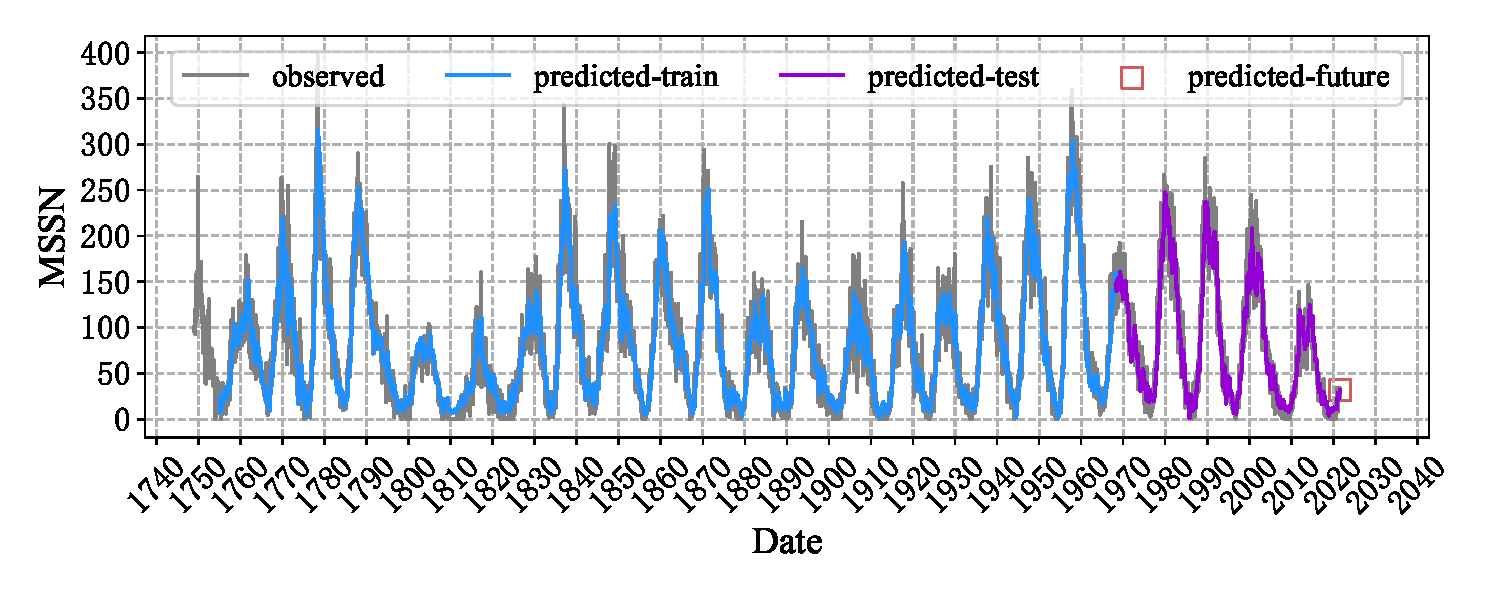
\includegraphics[width=\textwidth]{Img/chap5_ss/ssn_series_in_72_out_1_cnn.pdf}
    \label{fig:ssn_series_in_72_out_1_cnn}
  \end{subfigure} \\
  \vspace{-1cm}
  \begin{subfigure}[b]{1.0\textwidth}
    \caption{LSTM-1DCNN}
    \vspace{-0.35cm}
    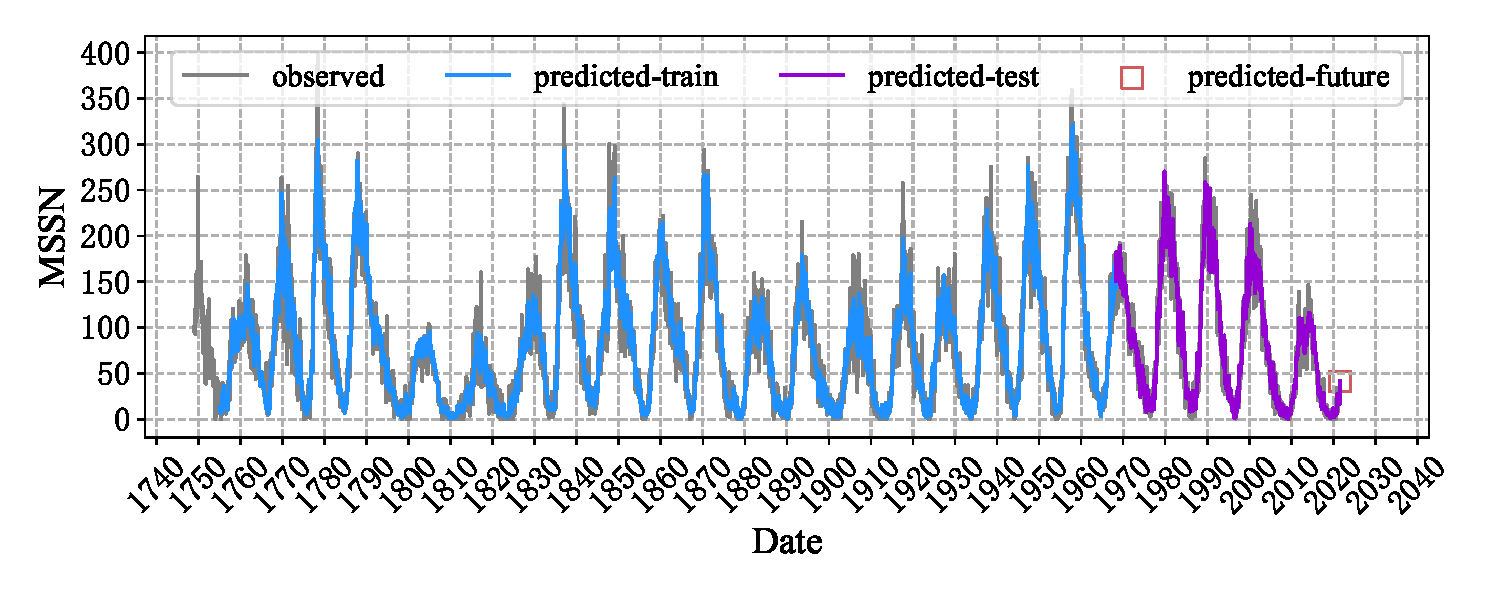
\includegraphics[width=\textwidth]{Img/chap5_ss/ssn_series_in_72_out_1_lstm_cnn.pdf}
    \label{fig:ssn_series_in_72_out_1_lstm_cnn}
    \end{subfigure}
  \vspace{-2cm}
  \bicaption{最佳模型预测未来1个月的太阳黑子数。}{Predicting the next monthly sunspot numbers by the best models.}
  \label{fig:ssn_series_in_72_out_1}
\end{figure}

讨论输出时间窗口为1个月的太阳黑子面积。表\ref{tab:ss_area_out_1}展示了使用不同模型(LSTM-RNN、1DCNN和LSTM-1DCNN)、不同输入窗口(1、72、132、264)未来1个月太阳黑子面积效果指标。表\ref{tab:ss_out_1}第二行展示了预测的未来太阳黑子面积。就网络性能而言,LSTM-1DCNN性能略优于LSTM-RNN和1DCNN。就输入窗口而言,历史132个月的太阳黑子面积作为时间窗口所得到的模型是最优的。当输入时间窗口为132个月$O_{-132}$时,LSTM-RNN的拟合指标为MSE$=\SI{0.0021}{}$, RMSE$=\SI{0.0463}{}$,预测2021年9月的太阳黑子面积为$\SI{274.1390}{}$;1DCNN的拟合指标为MSE$=\SI{0.0028}{}$, RMSE$=\SI{0.0531}{}$,预测2021年9月的太阳黑子面积为$\SI{359.7821}{}$;LSTM-1DCNN的拟合指标为MSE$=\SI{0.0021}{}$, RMSE$=\SI{0.0453}{}$,预测2021年9月的太阳黑子面积为$\SI{88.6146}{}$。

\begin{table}[!htbp]
  \centering
  \bicaption{不同模型、不同输入窗口预测未来1个月太阳黑子面积的测试集效果指标。}{The indicators of testing set for predicting the next monthly sunspot areas by different models with different input windows.}
  \label{tab:ss_area_out_1}
  \footnotesize
  \renewcommand{\arraystretch}{1}
  \begin{tabular}{ccccc}
    \toprule
    \multirow{2}{*}{模型} & \multirow{2}{*}{$I_{-k}$-[节点或过滤器数]-$O_{+f}$} & \multicolumn{2}{c}{验证集}\\
    \cmidrule(lr){3-4}
    \noalign{\smallskip}
    & & MSE & RMSE\\
    \midrule 
    LSTM-RNN & 1-[32]-1 & 0.0027 & 0.0521 \\
     & 72-[32]-1 & 0.0023 & 0.0483 \\
     & 132-[32]-1 & \textbf{0.0021} & \textbf{0.0463} \\
     & 264-[32]-1 & 0.0026 & 0.0507 \\
    \hline
    1DCNN & 72-[32]-1 & 0.0035 & 0.0588 \\
     & 132-[32]-1 & \textbf{0.0028} & \textbf{0.0531} \\
     & 264-[32]-1 & 0.0030 & 0.0551 \\
    \hline
    LSTM-1DCNN & 72-[64-32-16]-1 & 0.0021 & 0.0454 \\
     & 132-[64-32-16]-1 & \textbf{0.0021} & \textbf{0.0453} \\
     & 264-[64-32-16]-1 & 0.0023 & 0.0479 \\
    \bottomrule
\end{tabular}
\end{table}

\begin{figure}[!htbp]
  \centering
  \begin{subfigure}[b]{1.0\textwidth}
    \caption{LSTM-RNN} 
    \vspace{-0.35cm}
    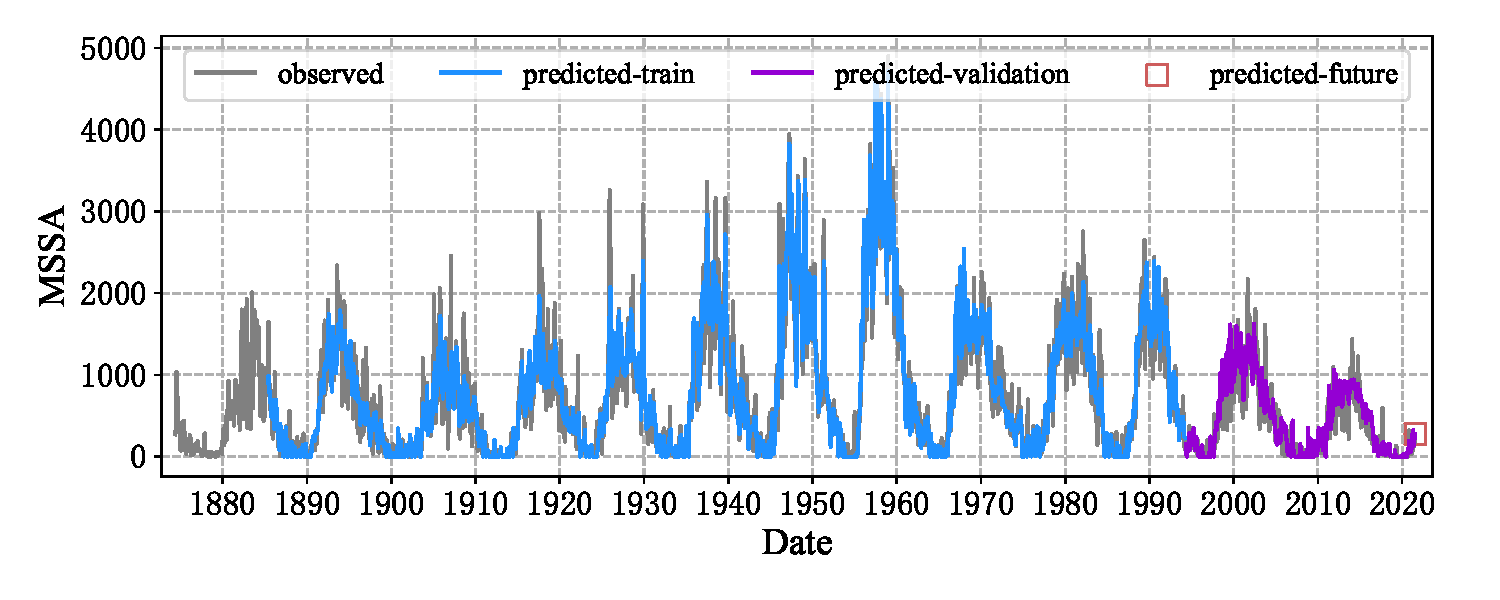
\includegraphics[width=\textwidth]{Img/chap5_ss/ssa_series_in_132_out_1_lstm.pdf}
    \label{fig:ssa_series_in_132_out_1_lstm}
  \end{subfigure}    \\
  \vspace{-1cm}
  \begin{subfigure}[b]{1.0\textwidth}
    \caption{1DCNN}
    \vspace{-0.35cm}
    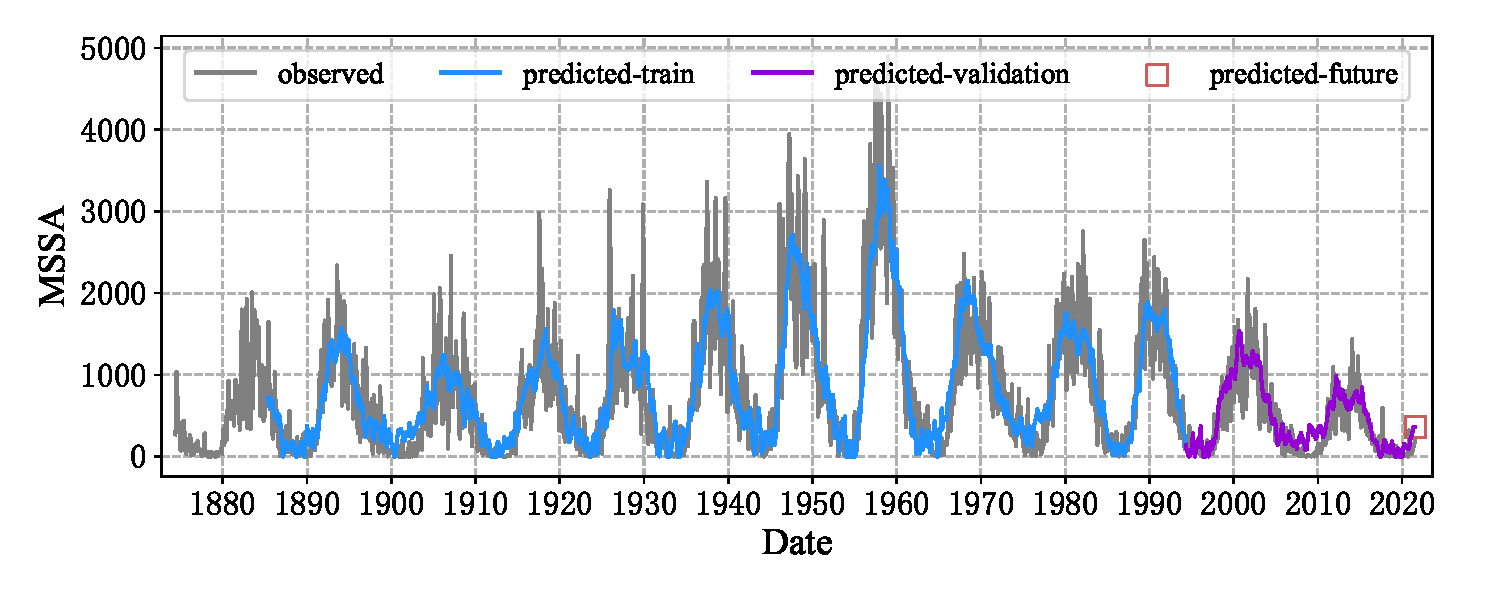
\includegraphics[width=\textwidth]{Img/chap5_ss/ssa_series_in_132_out_1_cnn.pdf}
    \label{fig:ssa_series_in_132_out_1_cnn}
  \end{subfigure} \\
  \vspace{-1cm}
  \begin{subfigure}[b]{1.0\textwidth}
    \caption{LSTM-1DCNN}
    \vspace{-0.35cm}
    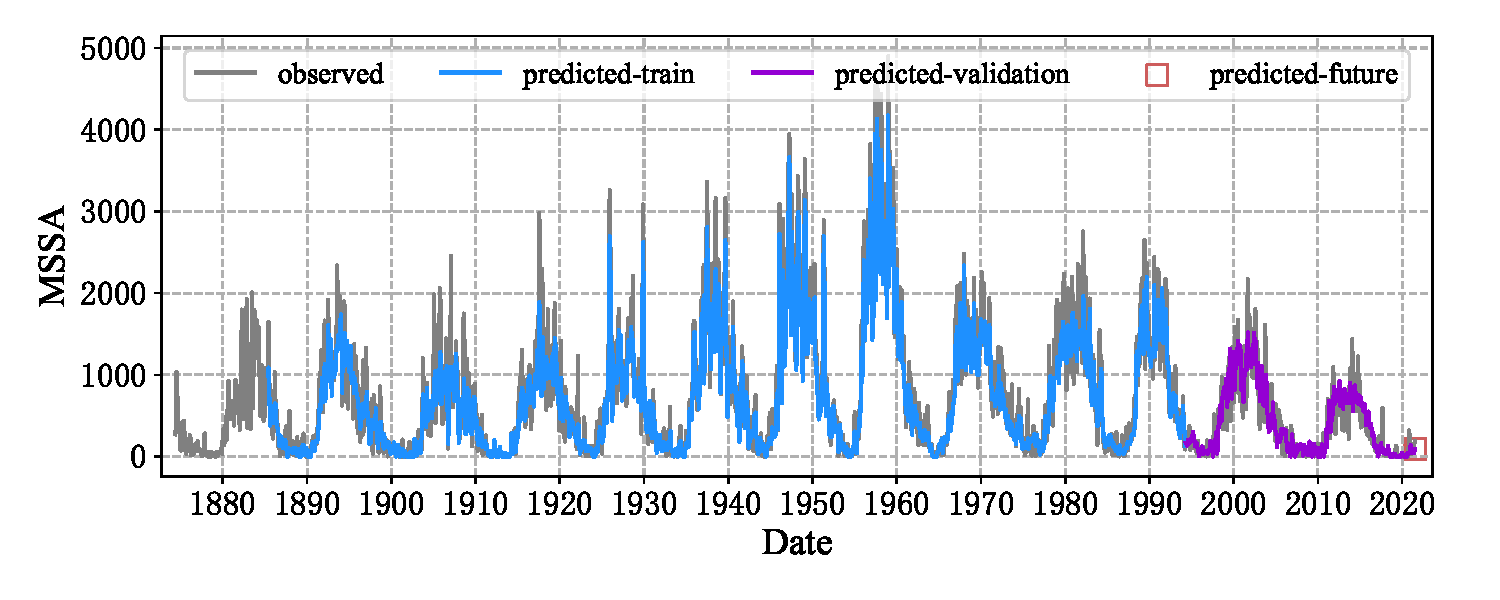
\includegraphics[width=\textwidth]{Img/chap5_ss/ssa_series_in_132_out_1_lstm_cnn.pdf}
    \label{fig:ssa_series_in_132_out_1_lstm_cnn}
    \end{subfigure}
  \vspace{-2cm}
  \bicaption{最佳模型预测未来1个月的太阳黑子面积。}{Predicting the next monthly sunspot areas by the best models.}
  \label{fig:ssa_series_in_132_out_1}
\end{figure}

\begin{table}[!htbp]
\centering
\bicaption{最佳模型预测2021年9月的太阳黑子强度。}{Prediction the sunspot amplitudes by the best models in September 2021.}
\label{tab:ss_out_1}
\footnotesize
\begin{tabular}{cccccc}
    \toprule
    日期 & 太阳黑子强度 & 输入时间窗口 & LSTM-RNN & 1DCNN & LSTM-1DCNN  \\
    \midrule
    2021年9月 & 数量 & 72个月 & 37.9250 & 31.6609 & 41.1549 \\
    2021年8月 & 面积 & 132个月 & 274.1390 & 359.7821 & 88.6146 \\
    \bottomrule
\end{tabular}
\end{table}

图\ref{fig:ssn_series_in_72_out_1}绘制了输入窗口为72的最佳模型预测未来1个月的太阳黑子数量,图\ref{fig:ssa_series_in_132_out_1}绘制了输入窗口为132的最佳模型预测未来1个月的太阳黑子面积。从图\ref{fig:ssn_series_in_72_out_1}和图\ref{fig:ssa_series_in_132_out_1}可以看出,对于预测值和测试集,LSTM-1DCNN具备良好的拟合能力。所有的结果均显示,预测的峰值比观测值略低,预测的谷值比观测值略高,这是因为太阳黑子强度较低或者较高,样本量偏少,模型难以准确学习到这些特征。


\subsection{预测未来72个月(半个太阳周)太阳黑子强度}\label{sec:ss_result_72}

第\ref{sec:ss_result_1}节,预测未来1个月太阳黑子数时,我们得出LSTM-1DCNN性能优于LSTM-RNN和1DCNN,因此以下试验不再考虑LSTM-RNN和1DCNN两种模型。本节讨论输出时间窗口为半个太阳周的太阳黑子强度。表\ref{tab:ss_number_out_72}展示了不同架构的LSTM-1DCNN模型、不同输入窗口(72、132、264)未来半个太阳周太阳黑子数量效果指标。与表\ref{tab:ss_number_out_1}相比,表\ref{tab:ss_number_out_72}中MSE值和RMSE值出现了一定程度的增加。也就是说,随着输出窗口的增加,模型性能会呈现下降趋势。该结论与泉流量中输出窗口对模型的影响类似。在相同的输入窗口条件下,隐藏层层数和节点数越多,MSE值越小,模型性能越好。就输入窗口而言,历史264个月的太阳黑子数量作为时间窗口所得到的LSTM-1DCNN模型是最优的。

表\ref{tab:ss_out_72}第一行展示了预测的未来72个月最大的太阳黑子数量及其发生时间。当输入时间窗口为264个月$O_{-264}$时,3层最佳的LSTM-1DCNN的拟合指标为MSE$=\SI{0.0085}{}$, RMSE$=\SI{0.0920}{}$,预测未来72个月的太阳黑子数最大值为$\SI{151.5516}{}$,,发生在2023年9月;4层最佳的LSTM-1DCNN的拟合指标为MSE$=\SI{0.0082}{}$, RMSE$=\SI{0.0905}{}$,预测未来72个月的太阳黑子数最大值为$\SI{174.7100}{}$,发生在2025年1月;5层最佳的LSTM-1DCNN的拟合指标为MSE$=\SI{0.0072}{}$, RMSE$=\SI{0.0849}{}$,预测未来72个月的太阳黑子数最大值为$\SI{132.8636}{}$,发生在2024年12月。对黑子数而言,第23太阳周最大MSSN出现在2001年9月,其值为238.2;第24太阳周最大MSSN出现在2014年2月,其值为146.1。我们的研究结果显示,第25太阳周的峰值跟第24太阳周基本持平。 

为了将可视化结果更清晰地展示,在展示训练集和测试集的结果时,只绘制了每个输入样本的第一个和最后一个预测值。图\ref{fig:ssn_series_in_264_out_72_lstm_cnn}绘制了不同结构的LSTM-1DCNN的最佳模型预测未来72个月的太阳黑子数。图\ref{fig:ssn_series_in_264_out_72_lstm_cnn}显示,未来第72个月超过了在第25太阳周的峰值。
图\ref{fig:ssn_series_in_264_out_72_layer_3_layersize_128_lstm_cnn}、图\ref{fig:ssn_series_in_264_out_72_layer_4_layersize_128_lstm_cnn}和图\ref{fig:ssn_series_in_264_out_72_layer_5_layersize_256_lstm_cnn}均在第25太阳周均出现了双峰性质,但图\ref{fig:ssn_series_in_264_out_72_layer_3_layersize_128_lstm_cnn}中的第一个峰值比第二个大,导致预测的峰值的时间提前到来。

\begin{table}[!htbp]
  \centering
  \bicaption{不同输入窗口和层数的LSTM-1DCNN预测未来72个月太阳黑子数量的测试集效果指标。}{The indicators of testing set for predicting the next 72 monthly sunspot numbers by LSTM-1DCNN with different input windows and layers.}
  \label{tab:ss_number_out_72}
  \footnotesize
  \renewcommand{\arraystretch}{1}
  \begin{tabular}{clccc}
    \toprule
    \multirow{2}{*}{层数} & \multirow{2}{*}{$I_{-k}$-[节点或过滤器数]-$O_{+f}$} & \multicolumn{2}{c}{验证集}\\
    \cmidrule(lr){3-4}
    \noalign{\smallskip}
    & & MSE & RMSE\\
    \midrule 
    3 & 72-[32(LSTM)-16(Conv)]-72 & 0.0189 & 0.1373 \\ 
      & 72-[64(LSTM)-32(Conv)]-72 & 0.0165 & 0.1283 \\
      & 72-[128(LSTM)-64(Conv)]-72 & 0.0140 & 0.1182 \\
      & 132-[32(LSTM)-16(Conv)]-72 & 0.0195 & 0.1397 \\
      & 132-[64(LSTM)-32(Conv)]-72 & 0.0124 & 0.1115 \\
      & 132-[128(LSTM)-64(Conv)]-72 & 0.0133 & 0.1151 \\
      & 264-[32(LSTM)-16(Conv)]-72 & 0.0155 & 0.1245 \\
      & 264-[64(LSTM)-32(Conv)]-72 & 0.0122 & 0.1103 \\
      & 264-[128(LSTM)-64(Conv)]-72 & \textbf{0.0085} & \textbf{0.0920} \\
    \hline
    4 & 72-[64(LSTM)-32(LSTM)-16(Conv)]-72 & 0.0179 & 0.1339 \\
      & 72-[128(LSTM)-64(LSTM)-32(Conv)]-72 & 0.0135 & 0.1162  \\
      & 72-[256(LSTM)-128(LSTM)-64(Conv)]-72 & 0.0146 & 0.1206 \\
      & 132-[64(LSTM)-32(LSTM)-16(Conv)]-72 & 0.0170 & 0.1305 \\
      & 132-[128(LSTM)-64(LSTM)-32(Conv)]-72 & 0.0132 & 0.1148 \\
      & 132-[256(LSTM)-128(LSTM)-64(Conv)]-72 & 0.0149 & 0.1220 \\
      & 264-[64(LSTM)-32(LSTM)-16(Conv)]-72 & 0.0089 & 0.0944 \\
      & 264-[128(LSTM)-64(LSTM)-32(Conv)]-72 & \textbf{0.0082} & \textbf{0.0905} \\
      & 264-[256(LSTM)-128(LSTM)-64(Conv)]-72 & 0.0093 & 0.0965 \\
    \hline
    5 & 72-[128(LSTM)-64(LSTM)-32(LSTM)-21(Conv)]-72 & 0.0173 & 0.1315 \\
      & 72-[256(LSTM)-128(LSTM)-64(LSTM)-42(Conv)]-72 & 0.0134 & 0.1157 \\
      & 72-[512(LSTM)-256(LSTM)-128(LSTM)-85(Conv)]-72 & 0.0158 & 0.1258 \\
      & 132-[128(LSTM)-64(LSTM)-32(LSTM)-21(Conv)]-72 & 0.0150 & 0.01226 \\
      & 132-[256(LSTM)-128(LSTM)-64(LSTM)-42(Conv)]-72 & 0.0163 & 0.1276 \\
      & 132-[512(LSTM)-256(LSTM)-128(LSTM)-85(Conv)]-72 & 0.0161 &  0.1268\\
      & 264-[128(LSTM)-64(LSTM)-32(LSTM)-21(Conv)]-72 & 0.0087 & 0.0935 \\
      & 264-[256(LSTM)-128(LSTM)-64(LSTM)-42(Conv)]-72 & \textbf{0.0072} & \textbf{0.0849} \\
      & 264-[512(LSTM)-256(LSTM)-128(LSTM)-85(Conv)]-72 & 0.0074 & 0.0859 \\
    \bottomrule
  \end{tabular}
\end{table}

\begin{figure}[!htbp]
  \centering
  \begin{subfigure}[b]{1.0\textwidth}
    \caption{264-[128(LSTM)-64(Conv)]-72} 
    \vspace{-0.35cm}
    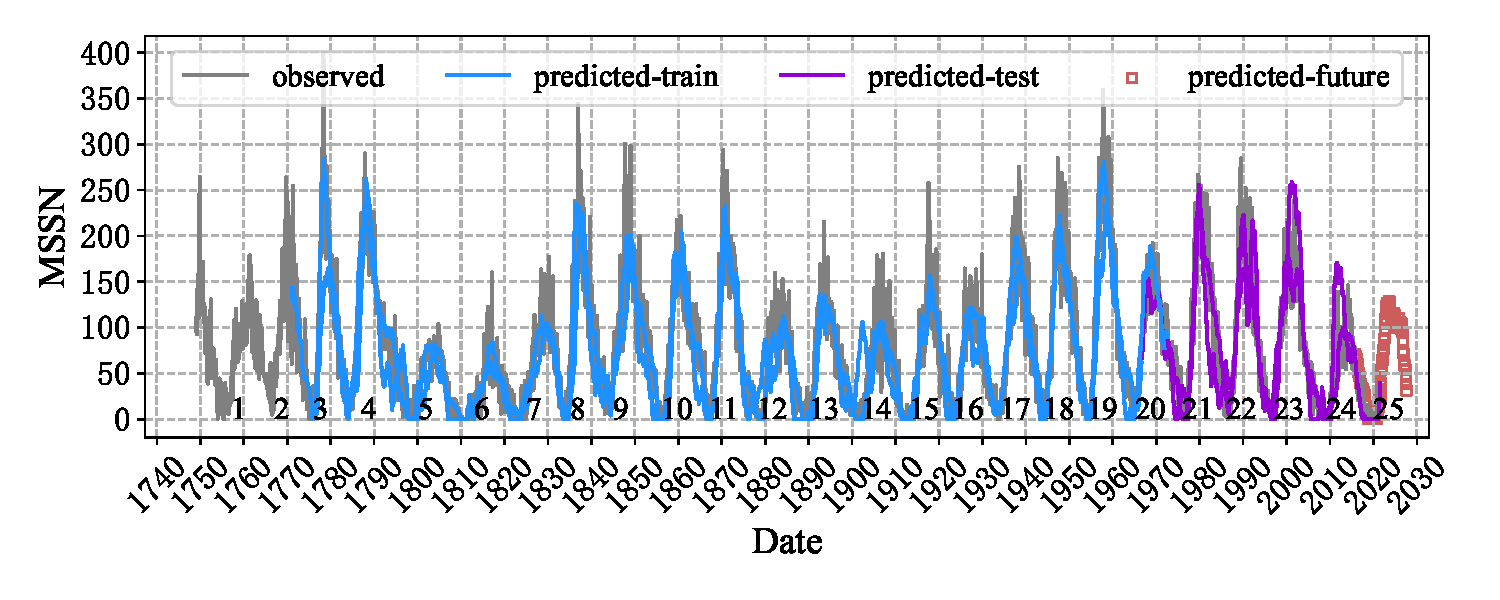
\includegraphics[width=\textwidth]{Img/chap5_ss/ssn_series_in_264_out_72_layer_3_layersize_128_lstm_cnn.pdf}
    \label{fig:ssn_series_in_264_out_72_layer_3_layersize_128_lstm_cnn}
  \end{subfigure}    \\
  \vspace{-1cm}
  \begin{subfigure}[b]{1.0\textwidth}
    \caption{264-[128(LSTM)-64(LSTM)-32(Conv)]-72}
    \vspace{-0.35cm}
    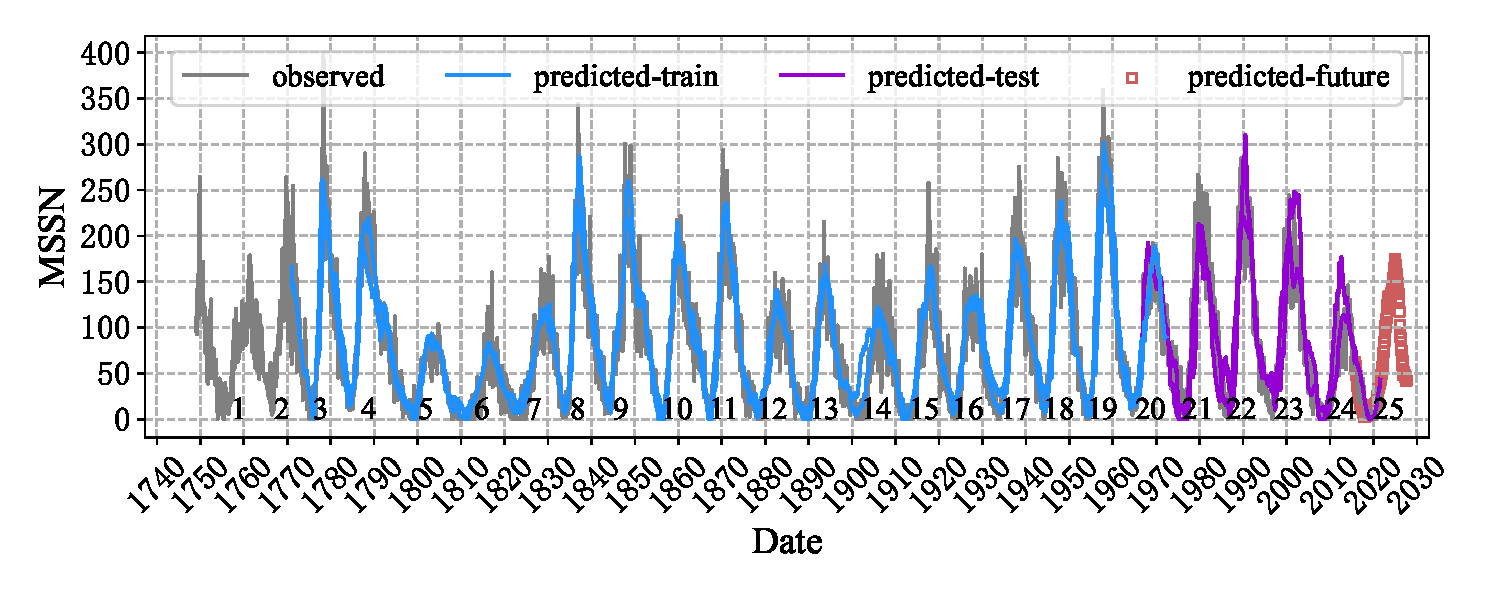
\includegraphics[width=\textwidth]{Img/chap5_ss/ssn_series_in_264_out_72_layer_4_layersize_128_lstm_cnn.pdf}
    \label{fig:ssn_series_in_264_out_72_layer_4_layersize_128_lstm_cnn}
  \end{subfigure} \\
  \vspace{-1cm}
  \begin{subfigure}[b]{1.0\textwidth}
    \caption{264-[256(LSTM)-128(LSTM)-64(LSTM)-42(Conv)]-72}
    \vspace{-0.35cm}
    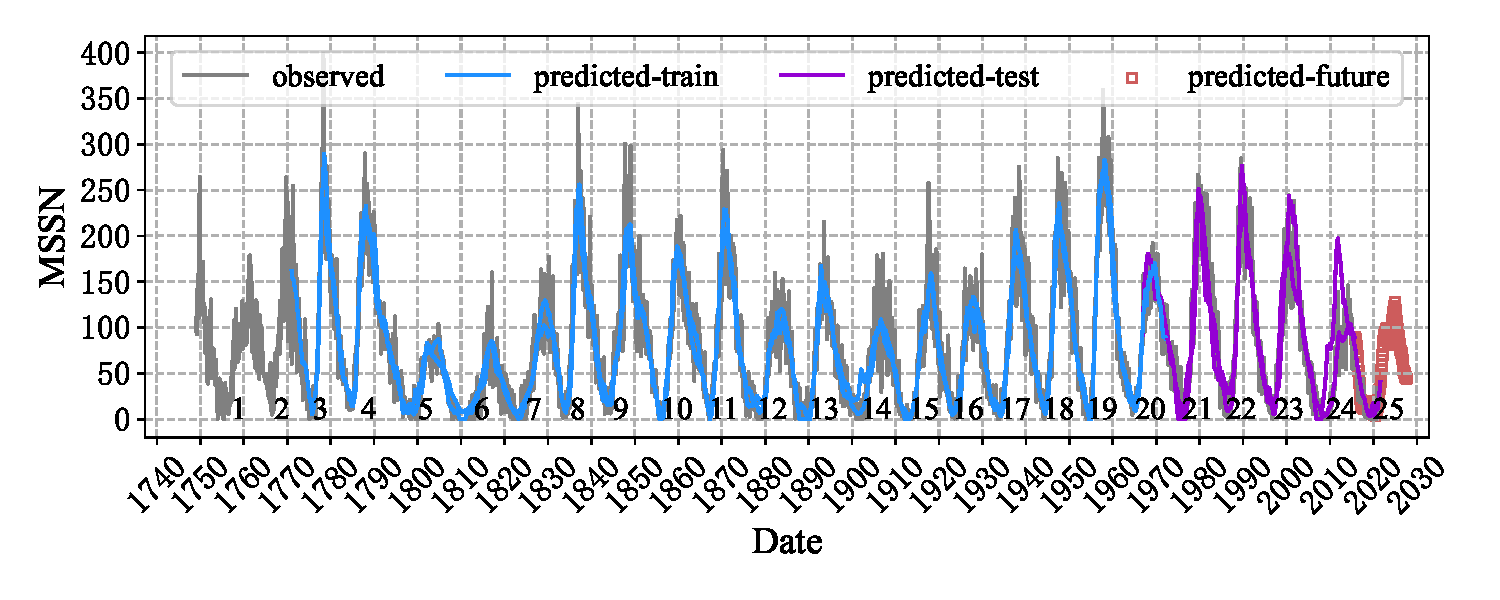
\includegraphics[width=\textwidth]{Img/chap5_ss/ssn_series_in_264_out_72_layer_5_layersize_256_lstm_cnn.pdf}
    \label{fig:ssn_series_in_264_out_72_layer_5_layersize_256_lstm_cnn}
    \end{subfigure}
  \vspace{-2cm}
  \bicaption{不同结构的LSTM-1DCNN的最佳模型预测未来72个月的太阳黑子数。}{Predicting the next 74 monthly sunspot numbers by the best LSTM-1DCNNs with different structure.}
  \label{fig:ssn_series_in_264_out_72_lstm_cnn}
\end{figure}

表\ref{tab:ss_out_72}第二行展示了预测的未来最大太阳黑子面积及其发生时间。3层最佳的LSTM-1DCNN模型的输入时间窗口为132个月$O_{-132}$时,的拟合指标为MSE$=\SI{0.0078}{}$, RMSE$=\SI{0.0884}{}$,预测未来72个月的太阳黑子面积最大值为$\SI{1016.323}{}$,,发生在2024年8月;4层最佳的LSTM-1DCNN的拟合指标为MSE$=\SI{0.0082}{}$, RMSE$=\SI{0.0905}{}$,预测未来72个月的太阳黑子面积最大值为$\SI{1469.0072}{}$,发生在2025年3月;5层最佳的LSTM-1DCNN的拟合指标为MSE$=\SI{0.0072}{}$, RMSE$=\SI{0.0849}{}$,预测未来72个月的太阳黑子面积最大值为$\SI{1397.7671}{}$,发生在2024年4月。对于太阳黑子面积,第23太阳周MSSA的峰值为2171.7,出现在2001年9月;第24太阳周MSSA的峰值为1439.82,出现在2014年2月。我们的研究结果显示,第25太阳周的峰值跟第24太阳周基本持平。 

为了将可视化结果更清晰地展示,在展示训练集和测试集的结果时,只绘制了每个输入样本的第一个和最后一个预测值。图\ref{fig:ssn_series_in_264_out_72_lstm_cnn}绘制了不同结构的LSTM-1DCNN的最佳模型预测未来72个月的太阳黑子数。图\ref{fig:ssn_series_in_264_out_72_lstm_cnn}显示,未来第72个月超过了在第25太阳周的峰值。
图\ref{fig:ssn_series_in_264_out_72_layer_3_layersize_128_lstm_cnn}、图\ref{fig:ssn_series_in_264_out_72_layer_4_layersize_128_lstm_cnn}和图\ref{fig:ssn_series_in_264_out_72_layer_5_layersize_256_lstm_cnn}均在第25太阳周均出现了双峰性质,但图\ref{fig:ssn_series_in_264_out_72_layer_3_layersize_128_lstm_cnn}中的第一个峰值比第二个大,导致预测的峰值的时间提前到来。

\begin{table}[!htbp]
  \centering
  \bicaption{不同输入窗口和层数的LSTM-1DCNN预测未来72个月太阳黑子面积的测试集效果指标。}{The indicators of testing set for predicting the next 72 monthly sunspot areas by LSTM-1DCNN with different input windows and layers.}
  \label{tab:ss_area_out_72}
  \footnotesize
  \renewcommand{\arraystretch}{1}
  \begin{tabular}{clccc}
    \toprule
    \multirow{2}{*}{模型} & \multirow{2}{*}{$I_{-k}$-[节点或过滤器数]-$O_{+f}$} & \multicolumn{2}{c}{验证集}\\
    \cmidrule(lr){3-4}
    \noalign{\smallskip}
    & & MSE & RMSE\\
    \midrule 
    3 & 72-[32(LSTM)-16(Conv)]-72 & 0.0105 & 0.1025 \\ 
      & 72-[64(LSTM)-32(Conv)]-72 & 0.0085 & 0.0923 \\
      & 72-[128(LSTM)-64(Conv)]-72 & 0.0097 & 0.0987 \\
      & 132-[32(LSTM)-16(Conv)]-72 & 0.0093 & 0.0965 \\
      & 132-[64(LSTM)-32(Conv)]-72 & 0.0091 & 0.0952 \\
      & 132-[128(LSTM)-64(Conv)]-72 & \textbf{0.0078} & \textbf{0.0884} \\
      & 264-[32(LSTM)-16(Conv)]-72 & 0.0091 & 0.0956 \\
      & 264-[64(LSTM)-32(Conv)]-72 & 0.0090 & 0.0950 \\
      & 264-[128(LSTM)-64(Conv)]-72 & 0.0084 & 0.0919 \\
    \hline
    4 & 72-[64(LSTM)-32(LSTM)-16(Conv)]-72 & 0.0107 & 0.1036 \\
      & 72-[128(LSTM)-64(LSTM)-32(Conv)]-72 & 0.0097 & 0.0986 \\
      & 72-[256(LSTM)-128(LSTM)-64(Conv)]-72 & 0.0099 & 0.0993 \\
      & 132-[64(LSTM)-32(LSTM)-16(Conv)]-72 & 0.0100 & 0.0998 \\
      & 132-[128(LSTM)-64(LSTM)-32(Conv)]-72 & 0.0091 & 0.0953 \\
      & 132-[256(LSTM)-128(LSTM)-64(Conv)]-72 & 0.0091 & 0.0953\\
      & 264-[64(LSTM)-32(LSTM)-16(Conv)]-72 & 0.0096 & 0.0978 \\
      & 264-[128(LSTM)-64(LSTM)-32(Conv)]-72 & 0.0075 & 0.0865 \\
      & 264-[256(LSTM)-128(LSTM)-64(Conv)]-72 & \textbf{0.0054} & \textbf{0.0733} \\
    \hline
    5 & 72-[128(LSTM)-64(LSTM)-32(LSTM)-21(Conv)]-72 & 0.0105 & 0.1023 \\
      & 72-[256(LSTM)-128(LSTM)-64(LSTM)-42(Conv)]-72 & 0.0071 & 0.0841 \\
      & 72-[512(LSTM)-256(LSTM)-128(LSTM)-85(Conv)]-72 & \textbf{0.0061} & \textbf{0.0781} \\
      & 132-[128(LSTM)-64(LSTM)-32(LSTM)-21(Conv)]-72 & 0.0089 & 0.0941 \\
      & 132-[256(LSTM)-128(LSTM)-64(LSTM)-42(Conv)]-72 & 0.0063 & 0.0791 \\
      & 132-[512(LSTM)-256(LSTM)-128(LSTM)-85(Conv)]-72 & 0.0067 & 0.0817 \\
      & 264-[128(LSTM)-64(LSTM)-32(LSTM)-21(Conv)]-72 & 0.0101 & 0.1006 \\
      & 264-[256(LSTM)-128(LSTM)-64(LSTM)-42(Conv)]-72 & 0.0075 & 0.0867 \\
      & 264-[512(LSTM)-256(LSTM)-128(LSTM)-85(Conv)]-72 & 0.0096 & 0.0980 \\
    \bottomrule
\end{tabular}
\end{table}

\begin{figure}[!htbp]
  \centering
  \begin{subfigure}[b]{1.0\textwidth}
    \caption{3层(132-[128(LSTM)-64(Conv)]-72)} 
    \vspace{-0.35cm}
    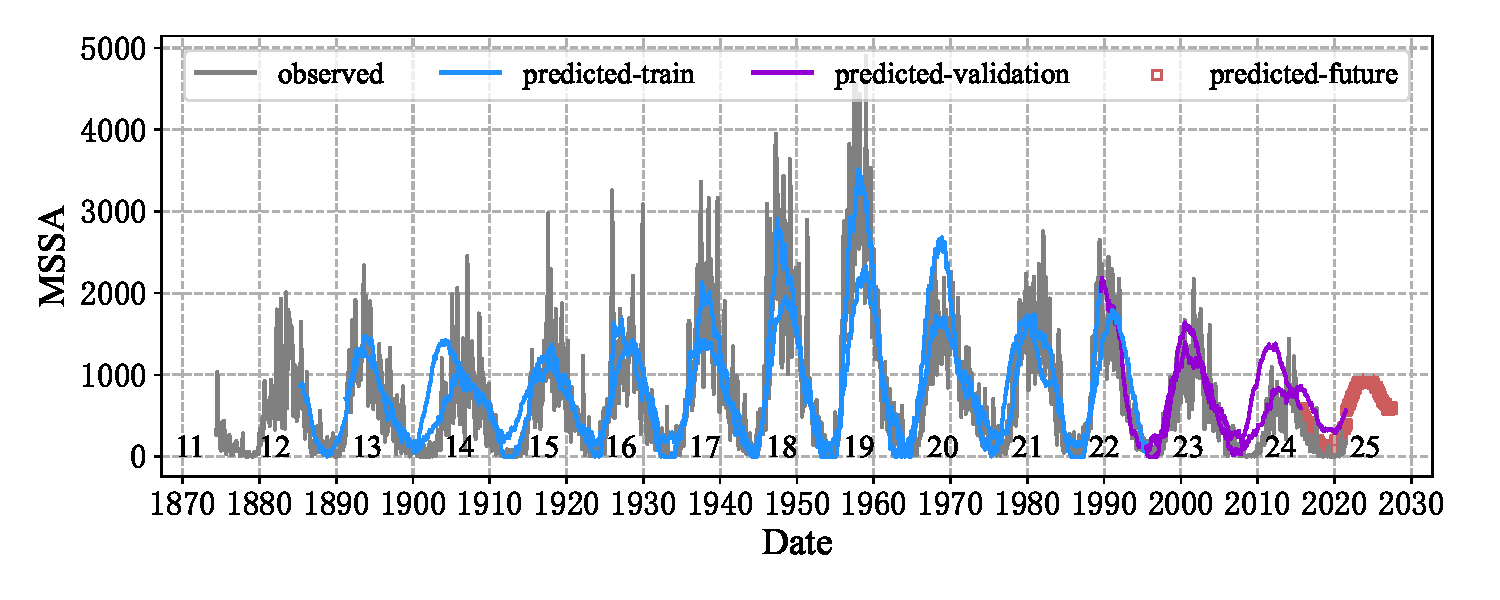
\includegraphics[width=\textwidth]{Img/chap5_ss/ssa_series_in_132_out_72_layer_3_layersize_128_lstm_cnn.pdf}
    \label{fig:ssa_series_in_132_out_72_layer_3_layersize_128_lstm_cnn}
  \end{subfigure}    \\
  \vspace{-1cm}
  \begin{subfigure}[b]{1.0\textwidth}
    \caption{4层(264-[256(LSTM)-128(LSTM)-64(Conv)]-72)}
    \vspace{-0.35cm}
    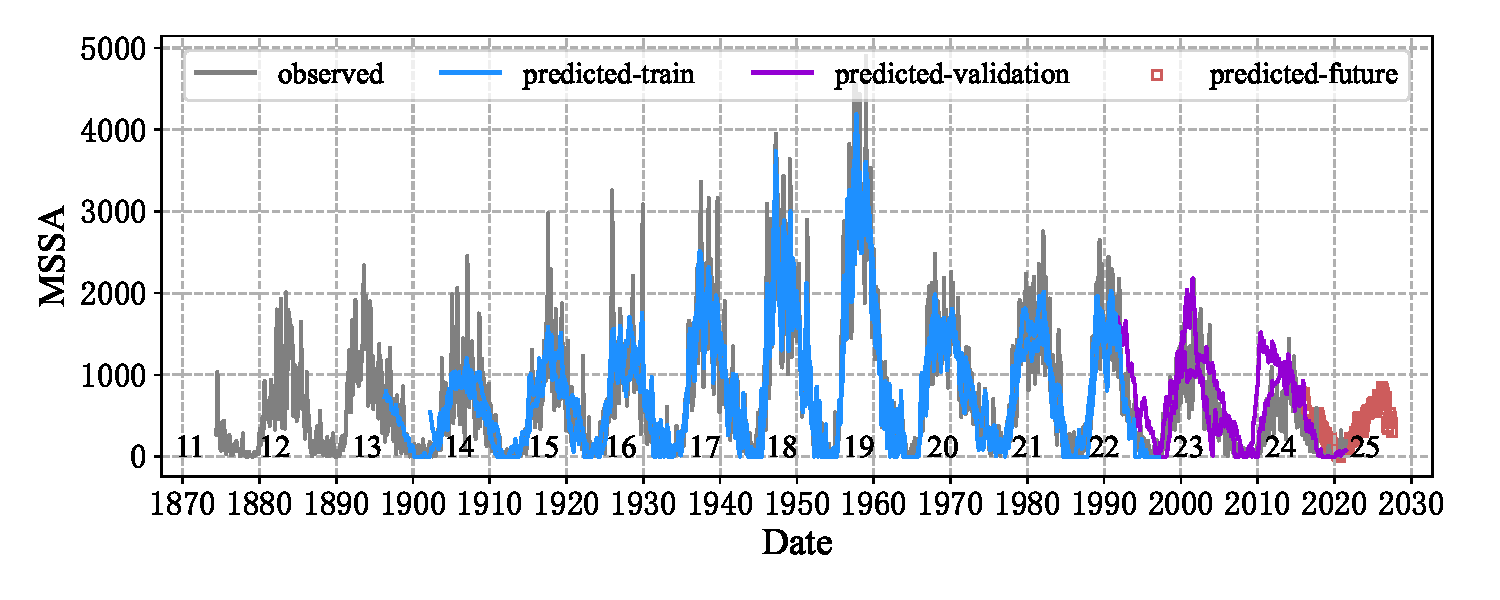
\includegraphics[width=\textwidth]{Img/chap5_ss/ssa_series_in_264_out_72_layer_4_layersize_256_lstm_cnn.pdf}
    \label{fig:ssa_series_in_264_out_72_layer_4_layersize_256_lstm_cnn}
  \end{subfigure} \\
  \vspace{-1cm}
  \begin{subfigure}[b]{1.0\textwidth}
    \caption{5层(72-[512(LSTM)-256(LSTM)-128(LSTM)-85(Conv)]-72)}
    \vspace{-0.35cm}
    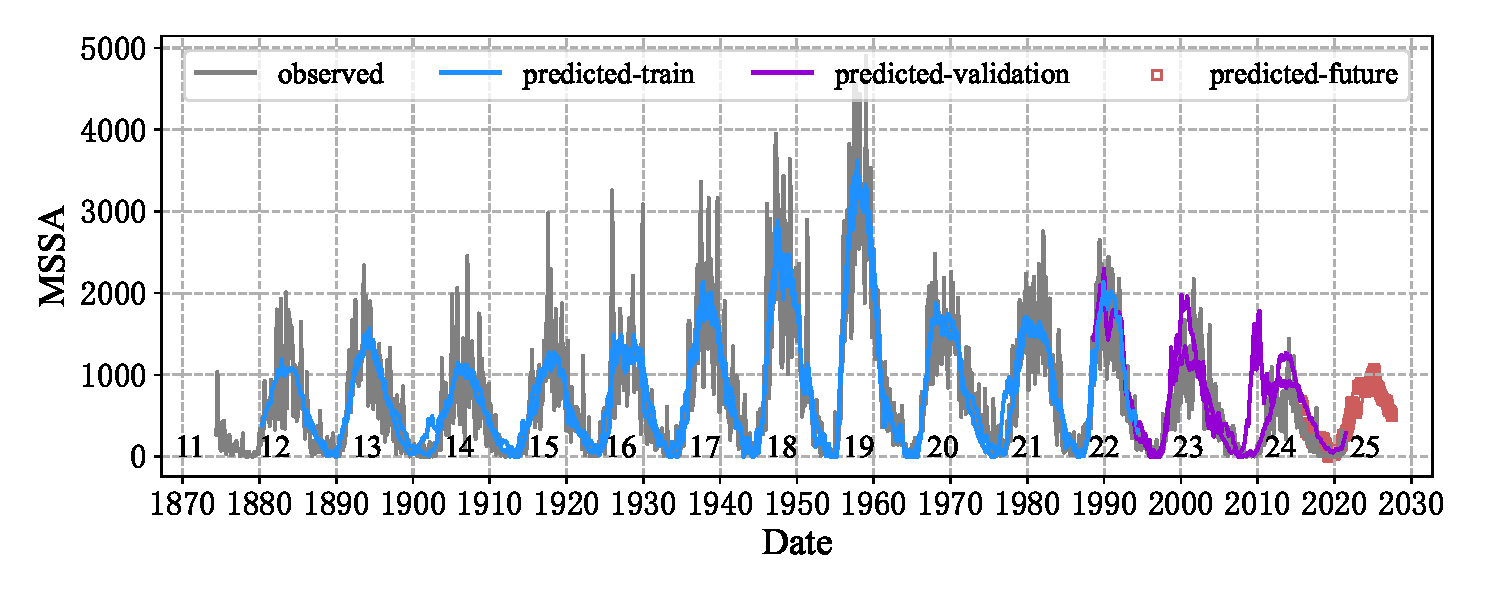
\includegraphics[width=\textwidth]{Img/chap5_ss/ssa_series_in_72_out_72_layer_5_layersize_512_lstm_cnn.pdf}
    \label{fig:ssa_series_in_72_out_72_layer_5_layersize_512_lstm_cnn}
    \end{subfigure}
  \vspace{-2cm}
  \bicaption{最佳模型预测未来72个月的太阳黑子面积。}{Predicting the next 72 monthly sunspot areas by the best models.}
  \label{fig:ssa_series_out_72_lstm_cnn}
\end{figure}

\begin{table}[!htbp]
\centering
\bicaption{最佳模型预测72个月峰值的太阳黑子强度。}{Prediction the sunspot maximum amplitudes by the best models in September 2021.}
\label{tab:ss_out_72}
\footnotesize
\begin{tabular}{cccccccc}
    \toprule
    &  & \multicolumn{2}{c}{3层} & \multicolumn{2}{c}{4层} & \multicolumn{2}{c}{5层}\\
    \cmidrule(lr){3-4} \cmidrule(lr){5-6} \cmidrule(lr){7-8}
    \noalign{\smallskip}
     & 输入窗口 & 最大值 & 发生时间 & 最大值 & 发生时间 & 最大值 & 发生时间 \\
    \midrule
    数量 & 264 & 151.5516 & 2023年9月 & 174.7100 & 2025年1月 & \textbf{132.8636} & \textbf{2024年12月} \\
    面积 & 132/264/72 & 1016.323 & 2024年8月 & \textbf{1469.0072} & \textbf{2025年3月} & 1397.7671 & 2024年4月 \\
    \bottomrule
\end{tabular}
\end{table}

图\ref{fig:ssn_series_in_264_out_72_lstm_cnn}和图\ref{fig:ssa_series_out_72_lstm_cnn}分别绘制了不同层数的最佳模型预测太阳黑子数量和面积。从图\ref{fig:ssn_series_in_264_out_72_lstm_cnn}和图\ref{fig:ssa_series_out_72_lstm_cnn}可以看出,对于预测值和测试集,LSTM-1DCNN具备良好的拟合能力。所有的结果均显示,预测的峰值比观测值略低,预测的谷值比观测值略高,这是因为太阳黑子强度较低或者较高,样本量偏少,模型难以准确学习到这些特征。

\subsection{与其他研究的比较}\label{sec:ss_result_compare}

已有很多研究中采取不同的方法预测即将到来的第25太阳周的太阳黑子变化,得到结果并不统一。原因可能是太阳黑子具备极其复杂的易变性、数据集长度的差异,预处理的差异,以及选择模型的差异等。表\ref{tab:ss_number_different_studies}列出部分关于第25太阳周的研究。例如,\citet{covas2019neural}使用具备时空特性的神经网络,预测第25太阳周可能是有史以来太阳黑子数最低的时期,预测峰值出现的时间为2022年至2023年。\citet{okoh2018hybrid}利用多维混合模型估计MSSN,得到第25太阳周的峰值为122.1(\pm 18.2),达到时间为2025年1月(\pm 6个月)。

\begin{table}[!htbp]
  \bicaption{不同研究给出的预测第25太阳周的太阳黑子。}{The different studies for predicting MSSN.}
  \label{tab:ss_number_different_studies}
  \centering
  \footnotesize
  \begin{tabular}{llll}
    \toprule 
    方法 & 相比第24太阳周 & 峰值达到时间 & 参考文献  \\
    \midrule
    LSTM-1DCNN & 基本相等 & 2024年12月-2025年3月 & 本研究 \\
    LSTM-RNN & 55\% 更强 & 2022年10月 & \citet{li2021predicting} \\
    前向传播神经网络 & 更弱 & 2022年至2023年左右 & \citet{covas2019neural} \\
    多维混合神经网络 & 基本相等 & 2025年1月(\pm 6个月)& \citet{okoh2018hybrid} \\
    光谱小波分解树 & 17\% 更强 & 2023年4月 & \citet{rigozo2011prediction} \\
    相似周期方法 & 30\% 更强 & 2024年10月& \citet{du2020solar} \\
    光谱分量外推法 & 29\% 更强 & 2022年至2023年之间 & \citet{kane2007solar}\\
    线性回归 & 10\%更强 & 2023年9月 & \citet{dani2019prediction}\\
    \bottomrule
\end{tabular}
\end{table}

\section{讨论与总结}\label{sec:ss_conclusion}

MSSN和MSSA时间序列数据是为非稳态的,数据中所包含的随机的分量使得太阳黑子在长时间预测尺度上不太可靠。由于数据中含有非线性效应的随机波动,难以对未来几个周期进行准确预测\citep{charbonneau2010dynamo,petrovay2010solar}。\citet{solanki2011analyzing}指出不同的关于长期预测太阳黑子变化研究得出的结论差异较大,这主要是因为太阳黑子变化具有非常复杂的非线性特征。\citet{charbonneau2010dynamo}认为,用于研究无法通过观察数据理解的物理系统的数学模型,不应上升为 "物理现实主义",因为模型难以反应现实。相较之下,太阳黑子活动起源于一定范围内的周期过程,而不是随机或间歇性过程\citep{mendoza2011mid}。

截至目前,太阳黑子预测最大的挑战是预测下一个周期的最大振幅和持续时间\citep{petrovay2010solar}。\citet{herrera2015reconstruction}假设太阳黑子每个周期存在一个固定的能量和给定频率(即太阳黑子活动周期在8年至14年之间),则太阳黑子估计模型的准确度会受到不确定原则的限制。因此,准确预测太阳黑子的任何参数(相位、振幅和周期)都十分困难。\citet{gleissberg1939long}曾指出太阳黑子周期的波动不够规则,在获取响应的表达函数时相当困难。不仅未来太阳周期的特性难以预测,而且准确预知太阳黑子数也几乎不可能。因此,太阳黑子周期预测的问题可以被视作一个概率问题。这也是太阳周期预测中经常会出现太阳黑子周期的预测概率。\citet{camporeale2019challenge}建议在空间天文研究中需要改变预测模式,从点预测到具有可靠不确定性的概率方法。找到并确认太阳周期磁力是预测第25太阳周的必要条件。太阳周期的振幅将取决于其在震荡阶段的位置变化。基于这一模式,理论上可以定性预测第25太阳周的最大振幅。然而,不同的物理模型和数值模型对于预测未来太阳周最大振幅还存在较大差异。根据120年太阳磁力模式的负向,第24太阳周可以归类为中度或较低的太阳活动。

本研究中,我们使用了LSTM-RNN、1DCNN以及两者的组合网络预测未来太阳黑子变化,采取的数据集是MSSN。第25太阳周,利用1DCNN预测的最大MSSN为157.80(发生在2025年1月),利用LSTM+1DCNN预测的最大MSSN为149.22(发生在2025年3月)。我们的预测结果与\citet{covas2019neural}的研究结果不仅在黑子强度上类似,而且在发生时间上也吻合。

% 另外,图\ref{fig:ssn_in132_out132_layer4_layer_size256}中,可以看出,不管是训练集、验证集,还是测试集,从完整的周期的角度看,每个周期均具有一定程度的双峰结构。最大振幅处呈现出水平变化,说明训练过的模型确实学到了双峰的特征。

% 当然本方法在太阳黑子预测上也存在局限性。从上面讨论可以看出,输入序列长度和输出序列长度直接决定了模型的构建,对预测结果有非常大的影响,这使得输入和输出序列长度成为好模型构建的一项前提条件。在前面分析过程中,输出长度越长,结果越不可靠。如果要提供非常准确的预报,可以将预报时长设置为1年,每隔一段时间更新模型,重新预测下一年的太阳黑子变化,这样也能为未来一年做准备。

% 除了时长的限制,第24太阳周的峰值和持续时间也发生了突变,这种突变会影响测试集的性能。图\ref{fig:ssn_in132_out132_layer4_layer_size256}(a)中,虽然1DCNN能够学习到第24太阳周的峰值,也能较好地拟合出双峰特征,但对于第24太阳周的持续时间,却做出了提前的预测。图\ref{fig:ssn_in132_out132_layer4_layer_size256}(b)中,虽然LSTM+1DCNN也能够学习到第24太阳周的峰值和准确预测第24太阳周的持续时间,但拟合出的双峰特征并不明显。因此,在使用过程中,我们可以结合两种方法做出判断。

